\hypertarget{aineisto-ja-menetelmuxe4t}{%
\chapter{Aineisto ja menetelmät}\label{aineisto-ja-menetelmuxe4t}}

\hypertarget{section}{%
\section{\texorpdfstring{\gls{ddd}}{}}\label{section}}

Yleinen ongelma tietokoneohjelmistoja tehtäessä on, että ohjelmoijat
tuntevat ohjelmiston erikoisalan heikosti. Esimerkiksi
kiinteistötekniikkaa, kirjastokortistoa tai tämän työn tapauksessa
terapiaklinikan toimintaa hoitavan ohjelmiston kehittäjä joutuu
käsittelemään monimutkaisia, sovellusalaan sidottuja ongelmia. Näiden
alojen asiantuntijat puolestaan tietävät, miten sovellusalan ongelmat
ratkaistaan, mutta heiltä puuttuu taito suunnitella ohjelmistoja.

Tämän ongelman ylittäminen on aihe, jota Eric Evans käsittelee kirjassan
Domain Driven Design. Evansin mielestä jokaisen monimutkaisemman
ohjelmiston sisässä on \gls{domainmodel} (Domain model), eli malli
siitä, miten kyseinen ohjelmisto ratkaisee sovellusalan ongelmat. Malli
voi kuitenkin olla piilotettu, ja saattaa olla, etteivät ohjelmiston
kehittäjät tiedosta mallin olemassaoloa. Tämän mallin tuominen näkyväksi
on \glsentryname{ddd}n päätavoite.

\Gls{crunching} (Knowledge crunching) on keskeinen väline
sovellusaluemallin rakentamiseen. Evans kuvaa prosessin, jossa
kehittäjät luonnostelevat yhdessä sovellusalueen asiantuntijoiden kanssa
\gls{domainmodel}in. Malli kytketään tiiviisti yhteen ohjelmakoodin
kanssa vuorottelemalla suunnittelun ja ohjelmistokehityksen välillä.
\cite[s. 13]{evans:ddd}

Tavoitteena on, että ohjelmistokehittäjien ja alan asiantuntijoiden
välille rakentuu \gls{ubilang}, jonka avulla kaikkien on mahdollista
yhteisesti keskustella ohjelmiston toiminnasta ja kehitystarpeista.
Tämän kielen käsitteet elävät ohjelmakoodissa, ja muodostavat koodin
ytimessä sijaitsevan \gls{domainlayer}

\hypertarget{n-rakennuspalikat}{%
\subsection{\texorpdfstring{\gls{ddd}n
rakennuspalikat}{n rakennuspalikat}}\label{n-rakennuspalikat}}

Evansin lähtökohta on, että \gls{domainmodel} ilmaistaan nimenomaan
ohjelmakoodin kautta. Koodi on kuitenkin lopulta se dokumentti, joka
määrittää ohjelman toiminnan.

Evans tarjoaa kirjassaan joukon käteviä työkaluja, joiden avulla
\glsentryname{domainmodel} on mahdollista toteuttaa teknisesti.

\Gls{entity} edustaa käytännössä kaikkea, jolla on identiteetti.
Esimerkiksi kahdella ihmisellä voi olla sama nimi, mutta he ovat silti
identiteetiltään eri henkilöitä. \gls{entity} voi myös muuttaa muotoaan,
esimerkiksi ihminen kasvaa aikuiseksi ja vaikkapa vaihtaa sukunimensä.
Identiteetti säilyy silti. Todella suuri osa
\glsentryname{domainmodel}{sta} koostuu juuri
\glsentryname{entity}{ista}.

Laskutusta käsittelevässä ohjelmassa esimerkiksi laskuilla on
identiteetti. Kahdella laskulla voi olla sisällytettynä samat tuotteet
ja maksajakin voi olla sama, mutta silti laskut ovat omia erillisiä
kokonaisuuksiaan.

Tärkeä osa mallia ovat myös olioiden väliset suhteet. Tosielämässä
kaikki liittyy kaikkeen, mutta sovellusalueen sisäinen logiikka
tarvitsee vain osajoukon kaikista suhteista toimiakseen. Huolellisesti
valitut suhteet olioiden välillä ilmaisevat enemmän mallin perimmäisestä
tarkoituksesta.

Myös \gls{kulkusuunta} \glsentryname{entity}{iden} välillä on tärkeä. Se
vaikuttaa paitsi ohjelmiston tekniseen monimutkaisuuteen, myös siihen,
minkälaisia asioita mallilla on mahdollista ilmaista.

Esimerkiksi lasku voi koostua joukosta laskurivejä. Ohjelman toteutus ja
käyttötavat muuttuvat hyvin paljon, jos kulkusuuntaa muutetaan.

\begin{itemize}
\tightlist
\item
  Tapaus A: lasku tietää, mitkä laskurivit siihen kuuluvat, mutta
  yksittäinen laskurivi ei tiedä, miltä laskulta on peräisin.
\item
  Tapaus B: laskurivi osaa kertoa, mille laskulle se kuuluu, mutta lasku
  ei kykene listaamaan omia rivejään.
\end{itemize}

Kolmas vaihtoehto on mahdollistaa kulkeminen molempiin suuntiin näiden
kahden käsitteen välillä. Tällöin ohjelman tekninen monimutkaisuus
kasvaa.

On tärkeää pyrkiä rajoittamaan olioiden väliset suhteet ja kulkusuunnat
mahdollisimman vähäisiksi, jotta ohjelma pysyy teknisesti mahdollisimman
yksinkertaisena.

Toisinaan sovellusalueeseen kuuluvat oliot muodostavat ryhmiä, joissa
yksi olio on juuriolio, ja muut riippuvat tästä. Tällaisia ryhmiä Evans
kutsuu nimellä \gls{aggregate}. Esimerkiksi laskurivi on hyödytön ilman
laskua, jolle se kuuluu. Lasku ja laskurivi muodostavatkin aggregaatin -
kokonaisuuden, jota käsitellään aina ryhmänä.

Kun monimutkaisempia sovellusalueen käsitteitä koostetaan, on toisinaan
hyödyllistä siirtää koostamistyö kokonaan erilliseksi oliokseen. Näitä
olioita Evans kutsuu tehdas-luokiksi (factory), samaan tapaan kuin
olio-ohjelmoinnin perinteessä muutenkin.

Tehdas-luokan tehtävänä on koostaa useasta alikäsitteestä koostuva
kokonaisuus.

Esimerkiksi laskulla voi olla maksaja, joukko laskutettavia asioita, ja
niitä vastaavat laskurivit ja juokseva numerointi. Tällaisen
kokonaisuuden rakentaminen ei enää onnistu yksinkertaisella laskun
luontikomennolla, vaan tarvitaan erillinen tehdas-luokka, jolta voi
pyytää eri tavoin rakennettuja laskuja.

\hypertarget{mallin-hiominen-refaktoroimalla}{%
\section{Mallin hiominen
refaktoroimalla}\label{mallin-hiominen-refaktoroimalla}}

Refaktoroinnilla tarkoitetaan koodin rakenteen muuttamista niin, että
koodin tuottama tulos ei muutu. Refaktoroimalla voi siistiä koodia ja
tehdä siitä luettavampaa.

Evansin mukaan hyvä \glsentryname{domainmodel} syntyy hyvin harvoin
ilman refaktorointia. Hän ei tarkoita refaktoroinnilla pelkästään koodin
teknistä siistimistä, vaan refaktoroinnin motivaationa on tuoda
\glsentryname{domainmodel} paremmin näkyviin koodin tasolla. Tämä vaatii
joustavasti kirjoitettua koodia, jota on helppo
muunnella.\cite[osa 3.]{evans:ddd}

Keskeinen keino joustavan koodin tuottamiseksi ovat edeltäkäsin
kirjoitettavat yksikkötestit. Kun testi laaditaan ennen koodin
kirjoittamista, koodin keskinäiset kytkökset muodostuvat löyhiksi.
Testien suoritustiheys on myös oleellista. Parhaisiin tuloksiin päästään
jatkuvalla testaamisella. Se on menetelmä, jossa testityökalu tarkkailee
lähdekooditiedostojen muutoksia, ja suorittaa testipatteriston uudelleen
joka kerta, kun koodiin tulee muutoksia. \cite[luku 6]{beck2004extreme}

Kattavasti yksikkötestattua koodia on myös helppo muunnella. Sen
rakenteeseen ja toimintaan voi tehdä suuriakin muutoksia, ilman että
tarvitsee pelätä takaiskuja. Tämä edellyttää, että testit ovat siistejä
ja vähäeleisiä, ja kirjoitettu samalla tarkkuudella kuin tuotantokoodi.
Paras metodi tähän tulokseen pääsemiseksi on kirjoittaa testejä ja
tuotantokoodia rinnakkain rivi riviltä. Ohjenuorana voi käyttää ns.
testipohjaisen kehittämisen kolmea
sääntöä.\cite[luku 9]{martin2008clean}

Joustavan järjestelmän suunnittelussa on myös hyvä seurata nk.
YAGNI-periaatetta. Kyseinen periaate edellyttää, että vain sellainen
koodi kirjoitetaan, jolle on tarvetta. Luokkiin tai moduuleihin ei
lisätä metodeita eikä toimintoja varmuuden varalta. \cite{jeffries1998}

Evans toteaa, että joustava rakenne on monesti seurausta siitä, että
\gls{domainmodel} kehittyy paremmaksi. Joustava ohjelmisto ei ole
monimutkainen, eikä se piilota toiminnallisuuksiaan outojen rajapintojen
taakse. Joustava ohjelmisto koostuu mahdollisimman pienestä määrästä
löyhästi toisiinsa kytkeytyviä käsitteitä.\cite[luku 10]{evans:ddd}

\hypertarget{graphql-teknologian-kuvaus}{%
\section{GraphQL-teknologian kuvaus}\label{graphql-teknologian-kuvaus}}

Monet web-sovellukset perustuvat \glsentryname{rest} (Representational
State Transfer) -rajapintoihin. \glsentryname{rest} on
arkkitehtuurityyli, jossa palvelin esittää asiakasohjelmalle joukon
resursseja, joita asiakasohjelma voi pyytää ja muunnella tilattomia
pyyntöjä käyttäen.\cite{fielding2000architectural}

REST-tyyli on vakiintunut web-sovellusten toteuttamisteknologiaksi,
mutta siihen liittyy myös eräitä ongelmia. Mikäli REST-tyyppisestä
rajapinnasta halutaan hakea usean eri resurssin verkko, joudutaan
tekemään erillinen pyyntö jokaista resurssia kohti. Toisissa tapauksissa
taas halutaan vain osa resurssin esittämästä tiedosta, mutta joudutaan
silti hakemaan koko
resurssi.\cite{betterRESTPrisma}\cite{WhyUseGraphQLApollo}

gls\{graphql\} on Facebookin kehittämä kyselykieli, joka on tarkoitettu
rajapintojen toteuttamiseen. Sen alkuperäinen suunnitteluperiaate oli
tarjota web-asiakasohjelmien kehittäjille aiempaa laajempi vapaus
rajapintapyyntöjen laatimiseen. \cite{graphql:spec}

GraphQL on vielä suhteellisen uusi teknologia, eikä siitä löydy kovin
paljoa materiaalia. Keskeinen tiedonlähde ovat Facebookin ja
GraphQL-säätiön julkaisemat verkkomateriaalit, sekä Apollo Graph
-yrityksen GraphQL-teknologiaa käsittelevä materiaali.

GraphQL koostuu kahdesta osasta: kyselykielestä sekä
tyyppijärjestelmästä. Kyselykielellä muotoillaan pyyntö, johon
GraphQL-palvelun tulee vastata.

GraphQL ei ole varsinainen rajapinta, sillä rajapinnan
toteuttamisteknologia on määrittelyn ulkopuolella. Useimmiten
GraphQL-palvelut on toteutettu \gls{http}-teknologian päälle, mutta
muitakin, kuten WebSocketia, voi käytttää. GraphQL ei myöskään
määrittele, miten kyselyn vastaus tulee muodostaa, tai milllä
ohjelmointikielellä järjestelmä tulee toteuttaa.

Osa konventioista on JavaScript-konventioita. Esimerkiksi kentän- ja
muuttujien nimet on tapana kirjoittaa camelCase- ja PascalCase
-muodoissa.\cite{GraphQLSchemaBasics}

\hypertarget{verkoista}{%
\subsection{Verkoista}\label{verkoista}}

\gls{verkko} eli graafi on tietorakenne, joka koostuu N:stä solmusta ja
niitä yhdistävistä kaarista.\cite{pozrikidis2014introduction} Verkkojen
avulla on mahdollista esittää monenlaisia asioiden välisiä suhteita,
kuten esimerkiksi reittikartta usean kaupungin välisistä teistä.

Olio-ohjelmoinnin tyyli esittää ratkaistavan ongelmakentän olioiden
välisinä verkkoina. Ohjelmassa ei ole juuri lainkaan jaettua tilan
käsittelyä, vaan kaikki kaikki tai lähes kaikki ohjelman sisältämä tieto
on olioissa. Näin käsiteltävät ongelmakokonaisuudet saadaan jaettua
pienempiin, hallittavan kokoisiin osiin. \cite{booch2008object}

GraphQL:n avulla sovellusala on mahdollista esittää verkon muodossa
määrittelemällä GraphQL-skeema. Tämän avulla rajapinta tarjoaa
asiakasohjelmalle rakenteen, joka muistuttaa
olio-ohjelmointia.\cite{thinkingInGraphs}

Juuri verkkorakenne tekee olio-ohjelmoinnista tehokkaan välineen
tosielämän ongelmien ratkaisemiseen. Oliot voivat edustaa ohjelman
\gls{domainmodel}n käsitteitä, ja verkko muodostaa niiden välisen
käsitekartan.

Käsitteiden verkkoa kuvaa myös Eric Evans Domain Driven Design
-kirjassa. Keino rakentaa \glsentryname{ubilang} kehittäjien ja alan
asiantuntijoiden välille on antaa tärkeille käsitteille nimet, sijoittaa
ne mallissa oikeisiin suhteisiin keskenään ja myös toteuttaa ne
koodissa.

\hypertarget{tyyppijuxe4rjestelmuxe4}{%
\subsection{Tyyppijärjestelmä}\label{tyyppijuxe4rjestelmuxe4}}

Tietokoneet käsittelevät dataa ottamatta sen enempää kantaa sen
\textbackslash{}gls{[}tyyppiin{]}\{tyyppi\}. Pohjimmiltaan data on vain
bittijonoja muistissa, tai elementtejä joukossa. Kun tällaista
järjestämätöntä ja tyypittämätöntä joukkoa ryhdytään käsittelemään, on
välttämätöntä järjestää se erilaisiin kategorioihin. Tämä tiedon
luokittelu synnyttää tyyppijärjestelmän, mutta järjestelmä ei ole
formaalisti määritelty, eikä tietokone voi niin ollen tehdä
tyyppitarkistusta.

Tyypitys tarkoittaa määrättyjä rajoituksia, joiden avulla voidaan
varmistaa muuttujan oikeellisuus. Staattinen tyypitys on menetelmä,
jossa ekspressioiden tyyppi voidaan määrittää staattisen analyysin
avulla, siis jo käännösaikaisesti. Vahva tyypitys taas mahdollistaa
tyypin tarkistamisen luotettavasti ajon aikana.
\cite{Cardelli+Wegner:1985}

GraphQL-rajapinta koostuu tyypeistä, joita rajapinnalle lähetettävä
kysely käyttää. Kyselyssä määritetään pyydettävät tyypit ja niiden
kentät. Rajapinta palauttaa takaisin oliota edustavan joukon kenttiä
\gls{hakurakenne}-muodossa. \cite{graphql:spec}

GraphQL:ää käyttävät sovellukset on kuitenkin useimmiten kirjoitettu
dynaamisesti tyypitetyillä kielillä. Esimerkiksi alkuperäinen
GraphQL-referenssi-implementaatio on kirjoitettu
JavaScriptillä.\cite{graphqlRefImple2021Oct}

Samoin Python-kieli on dynaamisesti tyypitetty, ja olioiden
tunnistamisessa se käyttää duck-tyypitykseksi kutsuttua menetelmää.
Duck-tyypityksessä olion tyyppiä ei tarkasteta välttämättä edes
ajonaikaisesti, vaan oletetaan sen sisältämien jäsenten
perusteella.\cite{pythonGloss2021Oct} Jos esimerkiksi oliosta löytyvät
kentät \emph{summa} ja \emph{laskunumero}, oletetaan, että olio on
lasku.

Tässä mielessä voidaan ajatella, että GraphQL on keino tuoda
ajonaikaisia tyyppitarkistuksia myös dynaamisesti tyypitetyillä kielillä
kirjoitettuun sovellukseen. Rajapinta erottaa toisistaan ohjelmiston
taustaosan ja käyttöliittymän, joten tällä rajalla tehtävän
tyyppitarkistuksen voi ajatella ehkäisevän virheitä ja parantavan
ohjelmiston luotettavuutta.

Oheisessa esimerkissä kuvaan rajapinnan edustamien tyyppien, ja sitä
myötä sen palauttamien olioiden väliset suhteet.
ConsolidatedInvoice-tyyppisessä oliossa on sisällä invoices-kenttä, joka
on lista Invoice-tyyppisiä olioita.

Laskutuksessa ConsolidatedInvoicella eli koontilaskulla tarkoitetaan
yhdistelmälaskua, joka kokoaa yksittäisiä laskuja (Invoice).

Tältä rajapinnalta voi pyytää listaa koontilaskuista. GraphQL:n
tyyppijärjestelmä takaa, että koontilaskun sisällä on invoices-jäsen,
joka sisältää listan Invoice-tyyppisiä olioita, eli siis laskuja.

\begin{verbatim}
type Query {
  consolidatedInvoices [ConsolidatedInvoice]
}

Type Invoice {
  number: Int
  sum: Float
  date: Date
}

type ConsolidatedInvoice {
  number: Int
  invoices: [Invoice]
}
\end{verbatim}

\hypertarget{skeema}{%
\subsection{Skeema}\label{skeema}}

\Gls{dsl} on ohjelmointikieltä korkeamman tason kieli, joka on
suunniteltu jollekin kapealle sovellusalueelle.\cite{landin1966next}
Esimerkkejä \glsentryname{dsl}istä ovat esimerkiksi UNIX-tyyppisistä
järjestelmistä tutut \emph{sed}- ja \emph{awk}-kielet. Tällaisen kielen
avulla on mahdollista määritellä monimutkaisiakin asioita
nopeasti.\cite{Raymond2003} Kieli tarjoaa tavanomaista ohjelmointikieltä
ilmaisuvoimaisemman ja täsmällisemmän tavan määritellä asioita.

Eräs täsmäkielen kanssa hyödynnettävä suunnittelumalli on kielen
käyttäminen tietorakenteiden abstraktioon.\cite{Spi00b}
GraphQL-rajapinnassa on kysymys juuri tästä.

GraphQL-rajapinnan tyypit, niille tehtävät kyselyt ja mutaatiot kuvataan
skeemassa, GraphQL-kielen avulla. Edellä esitetty ConsolidatedInvoice-
ja Invoice-olioista koostuva esimerkki on validi GraphQL-skeema. Tämä
skeemamäärittelyihin käytettävä kieli on riippumaton
ohjelmointikielestä.

GraphQL-kirjastot eri kielissä lukevat skeeman, tarkistavat sen, ja sen
jälkeen suorittavat Skeeman avulla ajonaikaisen tyyppitarkistuksen.

GraphQL-kehityksen tyylejä on useita, ja yksi suosittu tapa on
kirjoittaa skeema ensiksi. Se tarjoaa suuntaviivat sekä rajapinnan
tekniselle toteutukselle, että myös graafisen asiakasohjelman
laatimiselle.\cite{SchemaDriven2017Nov},\cite{SchemaDrivenDesign2021Jul}

GraphQL-skeemaa voi siis verrata Eric Evansin esittämään ajatukseen
\glsentryname{ubilang}sta. Esimerkiksi GraphQL Foundationin
materiaaleissa esitetään, että GraphQL-skeemaa tulisi ajatella jaettuna
kielenä oman ohjelmointitiimin kesken, ja myös käyttäjien kanssa
kommunikoimiseen.\cite{thinkingInGraphs}

\hypertarget{miten-graphql-sovellus-toimii}{%
\subsection{Miten GraphQL-sovellus
toimii}\label{miten-graphql-sovellus-toimii}}

\begin{figure}
\centering
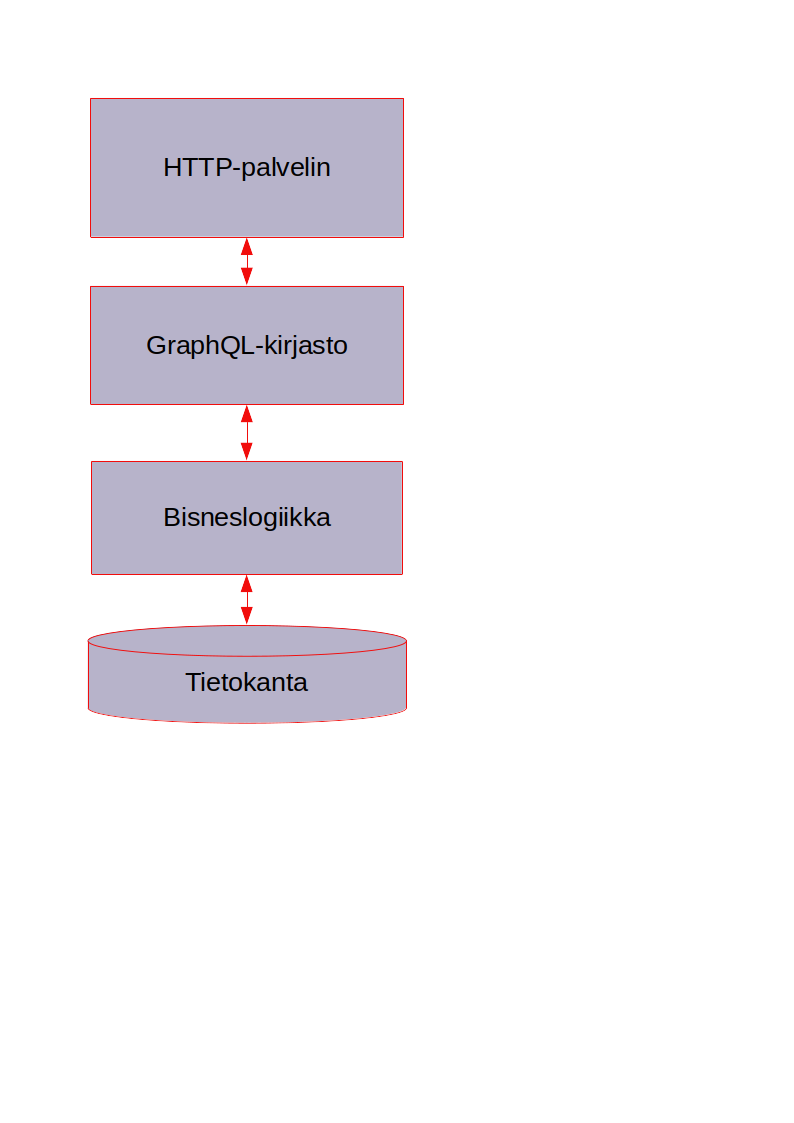
\includegraphics[width=\textwidth,height=0.5\textheight]{illustration/GraphQL-arkkitehtuuri.png}
\caption{\label{graphqlarkkitehtuuri} Esimerkkiarkkitehtuuri
GraphQL-sovellukselle}
\end{figure}

Kuvassa \ref{graphqlarkkitehtuuri} esitän yksinkertaisen
GraphQL-sovelluksen arkkitehtuurin. Arkkitehtuuri on kerroksittainen, ja
rajapinnalle esitettävä pyyntö liikkuu siinä ylhäältä alaspäin.

Ensiksi pyyntö saapuu HTTP-palvelimeen. Tämä palvelin on käytännössä
ohjelmointikielestä riippuen kirjasto, joka vastaanottaa HTTP-pyyntöjä
ja osaa käsitellä niitä. Tyypillisesti GraphQL-rajapinnassa on vain yksi
\texttt{graphql}-niminen resurssi, jolle pyynnöt esitetään.

HTTP-kerros ottaa pyynnön vastaan, ja lukee sen body-osassa olevan
merkkijonomuotoisen GraphQL-kyselyn. Tämä kysely on tehty
GraphQL-kyselykielellä. Rajapinta antaa kyselyn GraphQL-kirjastolle.

Kirjasto ottaa kyselyn vastaan, ja tarkistaa sen oikeellisuuden
GraphQL-skeemaa vasten. Mikäli kysely on muodoltaan oikeanlainen,
kirjasto ohjaa sen eteenpäin resolvereiksi kutsutuille funktioille.
Resolver-funktiot eivät ole osa kirjastoa, vaan sovelluksen kehittäjä
kirjoittaa ne. Käytännössä resolver-funktio on nk. \gls{puhdasfunktio},
jonka tehtävänä on tuottaa vastaus yksittäiseen GraphQL-kyselyn
kenttään.

Laskutusta käsittelevässä esimerkissä rajapinnan invoices-kenttää voisi
vastata \texttt{invoices\_resolver} -niminen funktio.

Resolver-funktioiden kerros on alin kerros, josta GraphQL-palvelu
tietää. Sen alla oleva ohjelmistologiikka on riippumaton rajapinnan
toteutustavasta. Tyypillisesti siellä voi sijaita sovelluksen
liiketoimintalogiikka ja infrastruktuuri, kuten esimerkiksi tiedon
tallennusteknologia.

\hypertarget{query-ja-mutation--juurityypit}{%
\subsection{Query ja Mutation
-juurityypit}\label{query-ja-mutation--juurityypit}}

GraphQL-palveluissa on muutama oletuksena määritelty tyyppi, joita
kutsutaan juurityypeiksi. Tässä käsittelen niistä kahta keskeisintä,
Query- ja Mutation-tyyppiä.

Rajapintaan voi tehdä kyselyjä Query-tyyppisen juuriolion kautta. Tämän
olion kentät määrittävät, mitä dataa rajapinnalta voidaan kysellä.
Kentät ovat ikäänkuin sisäänmenoaukkoja, joiden kautta oliorakenteita
voi pyytää.

Kun oheisen esimerkin mukaisesti määritellystä GraphQL-rajapinnasta
halutaan hakea tietoja, tehdään Query-tyypin consolidatedInvoices
-kenttään kysely, joka kuvaa halutun oliopuun rakenteen tyyppien avulla:

\begin{verbatim}
{
  consolidatedInvoices {
    number
    invoices {
      number
      sum
    }
  }
}
\end{verbatim}

Kyselyssä\ref{testfoo} määritellään kentät, jotka palautuvassa datassa
halutaan nähdä. Näin myös palautuvan oliopuun syvyyttä voidaan
kontrolloida. Oheisessa esimerkissä haetaan paitsi lista
koontilaskuista, myös jokaisen koontilaskun alle invoices-kenttään lista
siihen kuuluvista laskuista. Näin edetään verkkoa pitkin tarvittavan
datan luo.

Mutation-juurityyppiä puolestaan käytetään datan muunnoksiin.
Mutation-tyypin sisältämiin kenttiin lähetetään kysely, jossa mukana
olevat parametrit kertovat, miten dataa muokataan. Parametrit ovat yhtä
lailla tyypitettyjä kuin rajapinnan kentät, ja GraphLQ-kirjasto
tarkistaa niiden tyypin oikeellisuuden. Mutation-komennot voivat myös
palauttaa oliorakenteita.

Oheisessa esimerkissä määritellään invoice-niminen operaatio uuden
laskun luomiseen. Operaatiolle on merkitty paluuarvo, joka on
Invoice-tyypin olio. Käytännössä operaatio voisi siis palauttaa juuri
luodun laskun.

\begin{verbatim}
Mutation {
  invoice(customerId: Int, appointmentDate: String): Invoice
}
\end{verbatim}

Kun tällaista mutaatiota käytetään, kutsuun liitetään myös kyselyosa,
jossa listataan ne kentät, jotka palautuvasta oliosta halutaan. Tässä
tapauksessa pyydetään laskunumero ja laskun summa.

\begin{verbatim}
{
invoice(customerId: 1, appoitnmentDate: "2021-09-21") {
    number
    sum
  }
}
\end{verbatim}

\hypertarget{graphql-ja}{%
\section{\texorpdfstring{GraphQL ja
\glsentryname{ddd}}{GraphQL ja }}\label{graphql-ja}}

Eric Evansin kirjassa \glsentryname{domainmodel} rakennetaan
olio-ohjelmoinnin tekniikoita käyttäen. Vaikka se ei olekaan ainoa tapa
rakentaa \glsentryname{domainmodel}, on se kuitenkin tyylinä hyvin
suosittu.

Kuten edellä olen esittänyt, GraphQL puolestaan on olioverkkoon
perustuva rajapinta, jossa rajapinnan tarjoama tieto on jäsennetty
olioiksi ja niiden välisiksi suhteiksi.

Voidaan siis esittää kysymys, kuinka hyvin GraphQL-rajapinta soveltuu
\glsentryname{ddd} tarpeisiin? On helppo kuvitella, että olioverkolla on
mahdollista heijastaa \glsentryname{domainmodel}, ja jopa mallintaa se
lähes yksi yhteen. Toisaalta GraphQL-rajapinta palauttaa dataa, kun taas
olio-ohjelmoinnin keinon luotu olioverkko voi esittää dynaamisen ja
muuttuvan mallin. Onko GraphQL toimiva väline ohjelmiston tietomallin
parantamiseen? Tätä kysymystä lähden työni käytännön osassa
selvittämään.
